% ============================================================================
% Մանկավարժական լուծումներ - Դիսկրետ մաթեմատիկա, Գործնական 1 (Բազմությունների տեսություն).
% Խնդիրներ 2, 7, 11, 16, 20, 54(3,11), 58, 60. Հայերեն տարբերակ, XeLaTeX (fontspec + Sylfaen).
% Կազմել՝ xelatex-ով երկու անգամ։ Տերմինաբանությունը՝ glossary-ի համաձայն։
% ============================================================================
\documentclass[11pt,a4paper]{article}

% ---- Տառատեսակ (XeLaTeX) ----
\usepackage{fontspec}
\setmainfont{Sylfaen}

% Հայերենը plain XeLaTeX-ում տողադարձման կանոններ չունի, ուստի թող TeX-ը ձգի բացատները։
\tolerance=2000
\emergencystretch=3.5em

% ---- Մաթեմատիկա ----
\usepackage{amsmath,amssymb,amsthm}
\usepackage{mathtools}

% ---- Դասավորություն ----
\usepackage[margin=2.3cm]{geometry}
\usepackage{enumitem}
\usepackage{booktabs}
\usepackage{array}

% ---- Գրաֆիկա ----
\usepackage{xcolor}
\usepackage[most]{tcolorbox}
\usepackage{tikz}
\usetikzlibrary{arrows.meta,positioning,calc,fit,backgrounds,shapes.misc,shapes.geometric,decorations.pathreplacing}
\usepackage{pgfplots}
\pgfplotsset{compat=1.18}
\usepackage{hyperref}
\hypersetup{colorlinks=true,linkcolor=blue!55!black,urlcolor=blue!55!black}

% ---- Գունապնակ (Հայաստանի դրոշի գույները) ----
\definecolor{armRed}{HTML}{D90012}
\definecolor{armBlue}{HTML}{0033A0}
\definecolor{armOrange}{HTML}{F2A800}
\definecolor{ink}{HTML}{22303C}

\setlength{\parindent}{0pt}
\setlength{\parskip}{5pt}

% ---- Մաթ. կրճատումներ ----
\newcommand{\Z}{\mathbb{Z}}
\newcommand{\R}{\mathbb{R}}
\newcommand{\N}{\mathbb{N}}
\newcommand{\setdiff}{\setminus}
\DeclareMathOperator{\sd}{}
\newcommand{\symd}{\triangle}

% ---- Վանդակներ ----
\newtcolorbox{problembox}[1][]{enhanced, breakable, sharp corners=south,
  colback=armOrange!10, colframe=armOrange!75!black, boxrule=0.8pt, arc=2mm,
  fonttitle=\bfseries\color{white}, coltitle=white,
  attach boxed title to top left={xshift=4mm,yshift=-2.4mm},
  boxed title style={colback=armOrange!85!black, arc=1mm},
  title={Խնդիր #1}}

\newtcolorbox{ideabox}{enhanced, breakable,
  colback=armBlue!6, colframe=armBlue!70!black, boxrule=0.8pt, arc=2mm,
  fonttitle=\bfseries\color{white}, coltitle=white,
  attach boxed title to top left={xshift=4mm,yshift=-2.4mm},
  boxed title style={colback=armBlue!75!black, arc=1mm},
  title={Գաղափարը}}

\newtcolorbox{methodbox}{enhanced, breakable,
  colback=gray!8, colframe=gray!55!black, boxrule=0.7pt, arc=2mm,
  fonttitle=\bfseries, title={$\bigstar$\ Հիշարժան մեթոդ}}

\newtcolorbox{answerbox}{enhanced, sharp corners=south,
  colback=green!8, colframe=green!50!black, boxrule=1pt, arc=2mm, left=4mm,right=4mm}
\newcommand{\answer}[1]{\begin{answerbox}\centering\textbf{Պատասխան՝}\quad #1\end{answerbox}}

% ---- Վերնագիր ----
\title{\vspace{-1.2cm}\textbf{Դիսկրետ մաթեմատիկա - Գործնական 1}\\[2pt]
\large Բազմությունների տեսություն՝ մանրամասն լուծումներ\\[2pt]
\normalsize\itshape դատողությունները՝ քայլ առ քայլ բացված}
\author{}
\date{}

\begin{document}
\maketitle
\vspace{-1.0cm}

\begin{center}\small\itshape Ընդգրկում է Գործնական 1-ի հանձնարարված խնդիրները՝ 2, 7, 11, 16, 20, 54 (մասեր 3 և 11), 58, 60։\end{center}

\section*{Նախապատրաստում}

Այս թերթիկը հիմնականում բազմությունների պնդումներ \emph{ապացուցելու} մասին է, ոչ թե թվեր հաշվելու։
Հանդիպում է երեք տեսակի առաջադրանք։ (1) \textbf{Պատկանելության գլուխկոտրուկներ} (խնդիրներ 2, 7, 11)՝
պարզ պահիր $x$ տարրի և $\{x\}$ մեկտարրանոց բազմության տարբերությունը, որ պարունակում է այն՝ $\in$-ը և
$\subseteq$-ը տարբեր հարաբերություններ են։ (2) \textbf{Բազմությունների նույնություններ} (16, 20, 54,
60)՝ համընդհանուր գործիքը \emph{տարրային հետապնդումն} է՝ $X=Y$ ապացուցելու համար ցույց տուր, որ
կամայական տարր պատկանում է $X$-ին այն և միայն այն դեպքում, երբ պատկանում է $Y$-ին՝ վերագրելով սահմանող
պայմանը քայլ առ քայլ։ (3) Փոքր \textbf{կառուցման/կառուցվածքային} փաստարկ (58)։

Այստեղ օգտագործվող նշանակումները՝ $\overline{A}$-ն $A$-ի լրացումն է (ամեն ինչ $U$ ունիվերսալ
բազմությունում, որ $A$-ում չէ); $A\setminus B$-ն բազմությունների տարբերությունն է (աղբյուր թերթիկում
գրված է $A-B$); $A\symd B$-ն \emph{սիմետրիկ տարբերությունն} է (աղբյուրում գրված $\div$), սահմանված
որպես $A\symd B=(A\setminus B)\cup(B\setminus A)$; իսկ $\subset$-ը նշանակում է \emph{խիստ} պարունակում
($A\subseteq B$ և $A\neq B$), մինչդեռ $\subseteq$-ը թույլ է տալիս հավասարություն։

Այս թերթիկի ամենաօգտակար սովորությունը՝ երբ խրվում ես, իջիր մեկ տարրի մակարդակ։ Ստորև գրեթե
յուրաքանչյուր տող պարզապես «ի՞նչ է նշանակում ֆիքսված $x$-ի համար այստեղ պատկանելը» է։

% ============================================================================
\section*{Խնդիր 2 - Պատկանելության ո՞ր պնդումներն են ճիշտ}

\begin{problembox}[2]
Որոշիր, թե հետևյալներից որոնք են ճիշտ։
\begin{enumerate}[label=\textbf{2.\arabic*},leftmargin=2.2cm]
\item $\varnothing \in \{\varnothing,\ \{\varnothing\}\}$
\item $\{\varnothing\} \in \{\{\varnothing\}\}$
\item $\varnothing \in \{\{\varnothing\}\}$
\end{enumerate}
\end{problembox}

\begin{ideabox}
$x\in S$ ճիշտ է հենց այն դեպքում, երբ $x$-ը \emph{բառացիորեն $S$-ի ձևավոր փակագծերում թվարկված տարրերից
մեկն} է՝ ոչ ավելին։ Ուստի կարդա յուրաքանչյուր բազմությունը որպես ցանկ և հարցրու՝ արդյո՞ք ձախ կողմինը աջի
մուտքերից մեկն է։ Միակ որսն այն է, որ մուտքերն իրենք կարող են բազմություններ լինել, և չպետք է շփոթես
$\varnothing$-ը (դատարկ բազմությունը, $0$ տարր) $\{\varnothing\}$-ի հետ (արկղ, որ պարունակում է դատարկ
բազմությունը, $1$ տարր)։ Դրանք տարբեր օբյեկտներ են, ուստի $\varnothing\neq\{\varnothing\}$։ Վերաբերվիր
$\varnothing$-ին և $\{\varnothing\}$-ին որպես երկու տարբեր «անունների» և պարզապես սկանավորիր ցանկը։
\end{ideabox}

\textbf{Քայլ 1 - Թվարկիր յուրաքանչյուր աջ բազմության մուտքերը։}
\begin{itemize}[leftmargin=1.4cm]
\item $\{\varnothing,\ \{\varnothing\}\}$-ն ունի \emph{երկու} մուտք՝ $\varnothing$ և $\{\varnothing\}$։
\item $\{\{\varnothing\}\}$-ն ունի \emph{մեկ} մուտք՝ $\{\varnothing\}$։
\end{itemize}

\textbf{Քայլ 2 - Ստուգիր յուրաքանչյուր պնդումը ցանկի դեմ։}
\begin{itemize}[leftmargin=1.4cm]
\item \textbf{2.1} $\varnothing \in \{\varnothing,\{\varnothing\}\}$՝ արդյո՞ք $\varnothing$-ն երկու
մուտքերից մեկն է։ Այո, այն առաջինն է։ \textbf{Ճիշտ է։}
\item \textbf{2.2} $\{\varnothing\} \in \{\{\varnothing\}\}$՝ արդյո՞ք $\{\varnothing\}$-ն միակ
մուտքն է։ Այո, մուտքը հենց $\{\varnothing\}$ է։ \textbf{Ճիշտ է։}
\item \textbf{2.3} $\varnothing \in \{\{\varnothing\}\}$՝ արդյո՞ք $\varnothing$-ն միակ մուտքն է։ Միակ
մուտքը $\{\varnothing\}$ է, և $\varnothing\neq\{\varnothing\}$ (զրո տարր ընդդեմ մեկի)։ Ուստի՝ ոչ։
\textbf{Սխալ է։}
\end{itemize}

\textbf{Ստուգում։} Արագ ողջամտության ստուգում, որ 2.3-ն իսկապես սխալ է՝ $\{\{\varnothing\}\}$-ն ունի
ճիշտ մեկ տարր։ Եթե թե՛ $\varnothing$-ն, թե՛ $\{\varnothing\}$-ն պատկանեին նրան, այն կունենար երկու
տարբեր տարր։ Չունի, ուստի դրանցից առավելագույնը մեկն է նրանում՝ և 2.2-ն արդեն ճշտեց, որ դա
$\{\varnothing\}$-ն է։ \checkmark

\textbf{Երեք օբյեկտները որպես ներդրված արկղեր} (արկղը բազմություն է; նրա ներսում ազատ նստածներն իր
տարրերն են)։ Դրանք կողք կողքի կարդալը ցույց է տալիս, թե ինչու են բոլորը տարբեր՝

\begin{center}
\begin{tikzpicture}[font=\small,
  outer/.style={draw, thick, rounded corners=2pt, minimum width=2.7cm, minimum height=1.9cm},
  mid/.style={draw, armBlue!75!black, rounded corners=2pt, minimum width=1.5cm, minimum height=1.0cm},
  inn/.style={draw, armRed!75!black, rounded corners=2pt, minimum width=0.75cm, minimum height=0.5cm, fill=armRed!8}]
\node[outer, fill=gray!4] (o1) at (0,0) {};
\node[anchor=south] at (o1.north) {$\varnothing$};
\node[gray!60!black] at (o1) {\itshape (ներսում ոչինչ)};
\node[anchor=north, text width=2.9cm, align=center] at (o1.south) {$0$ տարր};
\node[outer, fill=gray!4] (o2) at (4.2,0) {};
\node[anchor=south] at (o2.north) {$\{\varnothing\}$};
\node[mid] (o2m) at (4.2,0.1) {$\varnothing$};
\node[anchor=north, text width=3.4cm, align=center] at (o2.south) {$1$ տարր՝ \ $\varnothing$};
\node[outer, fill=gray!4] (o3) at (8.4,0) {};
\node[anchor=south] at (o3.north) {$\{\{\varnothing\}\}$};
\node[mid, minimum width=1.7cm, minimum height=1.15cm] (o3m) at (8.4,0.05) {};
\node[inn] (o3i) at (8.4,-0.1) {$\varnothing$};
\node[anchor=south west, font=\tiny, armBlue!75!black] at (o3m.north west) {$\{\varnothing\}$};
\node[anchor=north, text width=3.6cm, align=center] at (o3.south) {$1$ տարր՝ \ $\{\varnothing\}$};
\end{tikzpicture}
\end{center}

\answer{2.1 Ճիշտ է, \quad 2.2 Ճիշտ է, \quad 2.3 Սխալ է։}

\begin{methodbox}
\textbf{Փոխանցելի տեխնիկա՝} $x\in S$-ը հարցնում է միայն «արդյո՞ք $x$-ը $S$-ի վերին մակարդակի ցանկի
տարր է»։ Մի՛ նայիր տարրերի ներսը։ Եվ միշտ $x$-ը առանձին պահիր $\{x\}$-ից՝ ինչ-որ բան ձևավոր փակագծերում
փաթաթելը ստեղծում է նոր, տարբեր օբյեկտ մեկ տարրով։
\end{methodbox}

% ============================================================================
\section*{Խնդիր 7 - $\in$-ը փոխանցական չէ}

\begin{problembox}[7]
Բեր $A,B,C$ բազմություններ՝ $A\in B$, $B\in C$, բայց $A\notin C$ պայմաններով։
\end{problembox}

\begin{ideabox}
$\le$ կամ $\subseteq$ տիպի հարաբերությունների համար շղթայումն աշխատում է՝ $a\le b\le c$ հարկադրում է
$a\le c$։ Այս վարժության իմաստն այն է, որ \emph{$\in$ պատկանելությունը չի շղթայվում}։ $A\in B$-ն ասում
է, որ $A$-ն մեկ մակարդակ ներքև է $B$-ի ներսում՝ $B\in C$-ն ասում է, որ $B$-ն մեկ մակարդակ ներքև է
$C$-ի ներսում, ուստի $A$-ն այժմ \emph{երկու} մակարդակ ներքև է $C$-ի ներսում՝ ինչը բոլորովին այլ պնդում
է, քան «$A$-ն $C$-ի տարր է»։ Սա զգալու ամենամաքուր ձևը աշտարակ կառուցելն է, որտեղ յուրաքանչյուր
բազմությունը ևս մեկ անգամ փաթաթված է ձևավոր փակագծերում։ Դասական աշտարակն է
$\varnothing,\ \{\varnothing\},\ \{\{\varnothing\}\}$։
\end{ideabox}

\textbf{Քայլ 1 - Ընտրիր աշտարակը։}
Դիցուք
$$A=\varnothing,\qquad B=\{\varnothing\},\qquad C=\{\{\varnothing\}\}.$$

\textbf{Քայլ 2 - Ստուգիր երկու պատկանելությունները։}
\begin{itemize}[leftmargin=1.4cm]
\item $A\in B$՝ արդյո՞ք $\varnothing$-ն $\{\varnothing\}$-ի մուտք է։ Այո։ \checkmark
\item $B\in C$՝ արդյո՞ք $\{\varnothing\}$-ն $\{\{\varnothing\}\}$-ի մուտք է։ Այո, այն միակ մուտքն է։ \checkmark
\end{itemize}

\textbf{Քայլ 3 - Ստուգիր չպատկանելությունը։}
$C=\{\{\varnothing\}\}$-ն ունի մեկ մուտք՝ $\{\varnothing\}$։ Արդյո՞ք $A=\varnothing$-ն այդ մուտքն է։
Ոչ, $\varnothing\neq\{\varnothing\}$։ Ուստի $A\notin C$։ \checkmark

\answer{$A=\varnothing,\quad B=\{\varnothing\},\quad C=\{\{\varnothing\}\}$։ \quad Սա վկայում է, որ $\in$-ը փոխանցական չէ։}

\medskip
\textbf{Ներդրման պատկերը} (յուրաքանչյուր արկղ մեկ մակարդակ է; $A$-ն թաղված է երկու մակարդակ խորը $C$-ի
ներսում, ուստի այն $C$-ի ուղիղ մուտք չէ)՝

\begin{center}
\begin{tikzpicture}[font=\small,
  lvl/.style={draw, rounded corners=3pt, inner sep=6pt}]
\node[lvl, fill=armBlue!8, minimum width=5.2cm, minimum height=2.6cm] (C) at (0,0) {};
\node[anchor=north west] at (C.north west) {\textbf{$C$}};
\node[lvl, fill=armOrange!12, minimum width=3.4cm, minimum height=1.5cm] (B) at (0.2,-0.15) {};
\node[anchor=north west] at (B.north west) {\textbf{$B$}};
\node[lvl, fill=armRed!12, minimum width=1.5cm, minimum height=0.7cm] (A) at (0.5,-0.3) {$A=\varnothing$};
\node[anchor=west] at (3.2,-0.15) {$A\in B,\ B\in C$};
\node[anchor=west] at (3.2,-0.75) {բայց $A\notin C$};
\end{tikzpicture}
\end{center}

% ============================================================================
\section*{Խնդիր 11 - Պարունակման/պատկանելության խառը շղթա}

\begin{problembox}[11]
Բեր $A,B,C,D,E$ բազմություններ՝ $A\subset B$, $B\in C$, $C\subset D$, $D\subset E$ պայմաններով, որտեղ
յուրաքանչյուր $\subset$ խիստ է։
\end{problembox}

\begin{ideabox}
Գլուխկոտրուկը խառնում է երկու տարբեր հարաբերություն մեկ շղթայում, և միակ անհարմար օղակը միջինն է՝
$B\in C$՝ այստեղ $B$-ն պետք է հանդես գա որպես $C$-ի ամբողջական \emph{տարր}, ոչ թե ենթաբազմություն։ Ուստի
կազմակերպիր $C$-ն այնպես, որ նրա թվարկված մուտքերից մեկը հենց $B$ բազմությունը լինի։ Մնացած ամեն ինչ
սովորական է՝ $X\subset Y$ խիստ պարունակման համար պարզապես վերցրու $Y$-ը որպես $X$՝ մեկ լրացուցիչ տարր
ավելացրած։ Նախ կառուցիր $A\subset B$, ապա $C$-ն դարձրու բազմություն, որ \emph{պարունակում է $B$-ն որպես
տարր}, ապա շարունակիր մեկ տարր ավելացնել՝ բարձրանալով $C\subset D\subset E$-ով։
\end{ideabox}

\textbf{Քայլ 1 - Խիստ $A\subset B$ զույգը։}
Վերցրու $A=\{1\}$ և $B=\{1,2\}$։ Այդ դեպքում $A\subseteq B$ և $A\neq B$, ուստի $A\subset B$ (խիստ)։ \checkmark

\textbf{Քայլ 2 - $B$-ն դիր որպես $C$-ի տարր։}
Մեզ պետք է, որ $B=\{1,2\}$-ն լինի $C$-ի \emph{մուտք}։ Վերցրու
$$C=\{\,\{1,2\},\,3\,\}.$$
Նրա երկու մուտքերն են $\{1,2\}$ բազմությունը և $3$ թիվը։ Քանի որ $\{1,2\}=B$-ն դրանցից մեկն է,
$B\in C$։ \checkmark
(Նկատի՛ր՝ սա պատկանելություն է, ոչ պարունակում՝ $B$-ն $C$-ի ներսում տարր է։)

\textbf{Քայլ 3 - Բարձրացիր խիստ պարունակումներով։}
Յուրաքանչյուր քայլում ավելացրու մեկ նոր տարր՝
$$D=\{\,\{1,2\},\,3,\,4\,\},\qquad E=\{\,\{1,2\},\,3,\,4,\,5\,\}.$$
Այդ դեպքում $C\subset D$ ($C$-ն ամբողջությամբ $D$-ում է, և $4\in D\setminus C$) և $D\subset E$ (և
$5\in E\setminus D$)։ Երկուսն էլ խիստ։ \checkmark

\textbf{Շղթան՝ $\in$-ը և $\subset$-ը տարբեր կերպ գծված։} Ներդրումը (մեկ օվալ/արկղ մյուսի ներսում)
նշանակում է $\subseteq$; բազմությունը՝ որպես մեկ \emph{ազատ տարր} ցանկում, նշանակում է $\in$։ Միակ
$\in$ օղակն այն է, որ $B$-ն հանդես է գալիս որպես $C$-ի մեկ տարր՝

\begin{center}
\begin{tikzpicture}[font=\footnotesize]
\node[draw, armBlue!75!black, ellipse, minimum width=3.0cm, minimum height=1.9cm, fill=armBlue!5] (Bset) at (0,0) {};
\node[anchor=north] at (Bset.north) {\color{armBlue!75!black}$B=\{1,2\}$};
\node[draw, armRed!75!black, ellipse, minimum width=1.5cm, minimum height=0.85cm, fill=armRed!8] (Aset) at (-0.35,-0.2) {$1$};
\node[anchor=south, font=\tiny, armRed!75!black] at (Aset.north) {$A=\{1\}$};
\node at (1.05,-0.25) {$2$};
\node at (0,-1.55) {$A\subset B$ (ներդրում)};
\node at (3.0,-0.2) {\large $\in$};
\node[anchor=south, font=\tiny] at (3.0,0.1) {որպես տարր};
\node[draw, thick, rounded corners=2pt, minimum width=3.3cm, minimum height=1.9cm, fill=gray!4] (Cset) at (5.6,0) {};
\node[anchor=north] at (Cset.north) {$C=\{\,B,\,3\,\}$};
\node[draw, armBlue!75!black, ellipse, minimum width=1.5cm, minimum height=0.85cm, fill=armBlue!12] (Bin) at (5.0,-0.25) {\scriptsize $\{1,2\}$};
\node[anchor=south, font=\tiny, armBlue!75!black] at (Bin.north) {$B$ (մեկ տարր)};
\node at (6.55,-0.3) {$3$};
\node at (5.6,-1.55) {$B\in C$ (պատկանելություն)};
\end{tikzpicture}

\medskip
\begin{tikzpicture}[font=\footnotesize,
  bx/.style={draw, thick, rounded corners=2pt, fill=gray!4}]
\node[bx, minimum width=6.2cm, minimum height=2.3cm] (E) at (0,0) {};
\node[anchor=north east] at (E.north east) {$E$};
\node[bx, minimum width=4.7cm, minimum height=1.7cm] (D) at (-0.35,-0.08) {};
\node[anchor=north east] at (D.north east) {$D$};
\node[bx, fill=armOrange!10, minimum width=3.2cm, minimum height=1.05cm] (C) at (-0.75,-0.18) {\scriptsize $\{\,B,\,3\,\}$};
\node[anchor=north east] at (C.north east) {$C$};
\node[anchor=west] at (2.6,0.35) {\scriptsize $4\in D\setminus C$};
\node[anchor=west] at (2.6,-0.35) {\scriptsize $5\in E\setminus D$};
\node[anchor=north] at (0,-1.25) {$C\subset D\subset E$ (ներդրում, յուրաքանչյուրն ավելացնում է մեկ տարր)};
\end{tikzpicture}
\end{center}

\answer{$A=\{1\},\ B=\{1,2\},\ C=\{\{1,2\},3\},\ D=\{\{1,2\},3,4\},\ E=\{\{1,2\},3,4,5\}$.}

\begin{methodbox}
\textbf{Փոխանցելի տեխնիկա՝} «$B\in C$» հարկադրելու համար թվարկիր $B$-ն ինքը որպես $C$-ի տարրերից մեկը
(մի՛ միաձուլիր $B$-ի տարրերը $C$-ի մեջ՝ դա կտար $B\subseteq C$)։ \emph{Խիստ} $X\subset Y$ պարունակում
հարկադրելու համար վերցրու $Y=X\cup\{\text{մեկ նոր տարր}\}$։
\end{methodbox}

% ============================================================================
\section*{Խնդիր 16 - Նկարագրիր ածանցյալ բազմությունները}

\begin{problembox}[16]
Դիցուք ունիվերսալ բազմությունը $U=\Z$ է, և
\begin{gather*}
A=\{x\in\Z:\exists y\in\Z^{+},\ x=2y\},\qquad
  B=\{x\in\Z:\exists y\in\Z^{+},\ x=2y-1\},\\
  C=\{x\in\Z:x<10\}.
\end{gather*}
Նկարագրիր $\overline{A}$, \ $\overline{A\cup B}$, \ $\overline{C}$, \ $A\setminus C$, \
$C\setminus(A\cup B)$ բազմությունները։
\end{problembox}

\begin{ideabox}
Նախ թարգմանիր յուրաքանչյուր սահմանող պայման պարզ բառերի, ապա մնացածն ամբողջ թվերի առանցքի վրա հաշվառում
է։ Քանի որ $y$-ը վերցնում է \emph{դրական} ամբողջ թվեր $\Z^{+}=\{1,2,3,\dots\}$՝
\begin{itemize}[leftmargin=1.2cm,topsep=2pt]
\item $x=2y$, $y\ge 1$-ով, տալիս է $A=\{2,4,6,\dots\}$՝ \textbf{դրական զույգ} ամբողջ թվերը։
\item $x=2y-1$, $y\ge 1$-ով, տալիս է $B=\{1,3,5,\dots\}$՝ \textbf{դրական կենտ} ամբողջ թվերը։
\item $C=\{x:x<10\}=\{\dots,7,8,9\}$՝ բոլոր ամբողջ թվերը $10$-ից \textbf{ներքև}։
\end{itemize}
Միակ դիտարկումը, որ մնացածը պարզ է դարձնում՝ յուրաքանչյուր դրական ամբողջ թիվ կա՛մ զույգ է, կա՛մ կենտ,
ուստի $A\cup B=\Z^{+}=\{1,2,3,\dots\}$։ $\overline{X}$ լրացումը «$U$ հանած $X$» է ($U=\Z$), իսկ
տարբերությունը «պահիր, ապա հեռացրու» է։ Դրանք թվային առանցքից կարդալը պատասխանները ակնհայտ է դարձնում։
\end{ideabox}

\textbf{Քայլ 1 - Երկու հիմնական միավորումները։}
$A\cup B$-ն բոլոր դրական զույգերն են բոլոր դրական կենտերի հետ միասին, այսինքն \emph{բոլոր դրական ամբողջ
թվերը}՝ $A\cup B=\Z^{+}=\{1,2,3,\dots\}$։

\textbf{Քայլ 2 - Կարդա յուրաքանչյուր բազմությունը։}
\begin{itemize}[leftmargin=1.4cm]
\item $\overline{A}=\Z\setminus\{2,4,6,\dots\}$՝ յուրաքանչյուր ամբողջ թիվ, որ \emph{ոչ} դրական զույգ է,
այսինքն բոլոր $x\le 0$ ամբողջ թվերը բոլոր դրական կենտերի հետ միասին
($\{\dots,-2,-1,0\}\cup\{1,3,5,\dots\}$)։
\item $\overline{A\cup B}=\Z\setminus\Z^{+}=\{0,-1,-2,\dots\}=\{x\in\Z:x\le 0\}$ (ոչ դրական ամբողջ
թվերը՝ զրո և բացասականները)։
\item $\overline{C}=\Z\setminus\{x<10\}=\{x\in\Z:x\ge 10\}=\{10,11,12,\dots\}$։
\item $A\setminus C$՝ դրական զույգեր, որ \emph{ոչ} $10$-ից ներքև են, այսինքն դրական զույգեր
$\ge 10$՝ $\{10,12,14,\dots\}$։
\item $C\setminus(A\cup B)$՝ $10$-ից ներքև ամբողջ թվեր՝ բոլոր դրական ամբողջ թվերը հեռացրած, թողնելով ոչ
դրականները՝ $\{0,-1,-2,\dots\}=\{x\in\Z:x\le 0\}$։ Սա \emph{նույն} բազմությունն է, ինչ
$\overline{A\cup B}$-ն (յուրաքանչյուր $x\le 0$ $10$-ից ներքև է, ուստի $\Z^{+}$-ը $\Z$-ից կամ
$\{x<10\}$-ից հեռացնելը թողնում է նույն բանը)։
\end{itemize}

\textbf{Ստուգում (թվային առանցք, պատուհան՝ $-3$-ից $12$)։}
Ստորև պատկերը հետևում է $A$-ին (դրական զույգեր) և $B$-ին (դրական կենտեր)։ Աչքով կարելի է ստուգել՝
$A\setminus C$-ն սկսում է $10$-ից; $\overline{C}$-ն ամեն ինչ է $10$-ից վեր; իսկ թե՛ $\overline{A\cup B}$-ն,
թե՛ $C\setminus(A\cup B)$-ն հենց $\le 0$ կետերն են։ $-20\le x\le 20$ վրայով ուղիղ թվարկումը հաստատում է
բոլոր հինգ նկարագրությունները և $C\setminus(A\cup B)=\overline{A\cup B}$ հավասարությունը։ \checkmark

\begin{center}
\resizebox{\textwidth}{!}{%
\begin{tikzpicture}[font=\footnotesize,>=Stealth]
\def\xlo{-3}\def\xhi{12}
\draw[<->] (\xlo-0.6,0) -- (\xhi+0.8,0) node[right]{$\Z$};
\foreach \x in {-3,...,12}{
  \draw (\x,0.08) -- (\x,-0.08);
  \node[below] at (\x,-0.1) {\tiny \x};
}
\draw[armOrange!80!black, dashed] (9.5,-0.5) -- (9.5,1.7);
\node[armOrange!70!black, anchor=south] at (9.5,1.7) {\tiny $x<10\ |\ x\ge 10$};
\foreach \x in {2,4,6,8,10,12}{
  \fill[armRed] (\x,0.55) circle (2.6pt);
}
\node[armRed, anchor=west] at (\xhi+0.2,0.55) {};
\node[armRed] at (\xlo-0.9,0.55) {\tiny $A$};
\foreach \x in {1,3,5,7,9,11}{
  \draw[armBlue, fill=white, line width=0.8pt] (\x,1.05) circle (2.6pt);
}
\node[armBlue] at (\xlo-0.9,1.05) {\tiny $B$};
\draw[decorate, decoration={brace, amplitude=4pt}, gray!60!black]
  (\xlo-0.55,-0.55) -- (0,-0.55);
\node[gray!60!black, anchor=north] at (-1.5,-0.62) {\tiny $\overline{A\cup B}=C\setminus(A\cup B)=\{x\le 0\}$};
\node[anchor=west] at (\xlo-0.6,1.7) {\tiny \textcolor{armRed}{$\bullet$} դրական զույգեր $A$\quad \textcolor{armBlue}{$\circ$} դրական կենտեր $B$};
\end{tikzpicture}%
}
\end{center}

\answer{$\overline{A}=\{x\le 0\}\cup\{1,3,5,\dots\}$;\quad
$\overline{A\cup B}=\{x\le 0\}=\{0,-1,-2,\dots\}$;\quad
$\overline{C}=\{10,11,12,\dots\}$;\quad
$A\setminus C=\{10,12,14,\dots\}$;\quad
$C\setminus(A\cup B)=\{x\le 0\}\ (=\overline{A\cup B})$.}

\begin{methodbox}
\textbf{Փոխանցելի տեխնիկա՝} նախ վերծանիր յուրաքանչյուր բազմություն-կառուցիչը մեկ պարզ նախադասության
(«դրական զույգեր», «$10$-ից ներքև ամբողջ թվեր»), նկատիր կառուցվածքային փաստը, որ ամեն ինչ պարզ է դարձնում
($A\cup B=\Z^{+}$), ապա կարդա լրացումները որպես «$U$ հանած բազմությունը» և տարբերությունները՝ որպես
«պահիր, ապա հեռացրու»։ Թվային առանցքը այն վերածում է մի բանի, որ պարզապես կարող ես նայել։
\end{methodbox}

% ============================================================================
\section*{Խնդիր 20 - Համարժեք պայմանների երեք ընտանիք}

\begin{problembox}[20]
Դիցուք $A,B$-ն $U$ ունիվերսալ բազմության կամայական ենթաբազմություններ են։ Ապացուցիր, որ յուրաքանչյուր
տողում թվարկված բոլոր պայմանները համարժեք են։
\begin{enumerate}[label=\textbf{Տող \arabic*՝},leftmargin=2cm]
\item $A\subseteq B\ \Longleftrightarrow\ \overline{B}\subseteq\overline{A}\ \Longleftrightarrow\
A\cup B=B\ \Longleftrightarrow\ A\cap B=A$.
\item $A\cap B=\varnothing\ \Longleftrightarrow\ A\subseteq\overline{B}\ \Longleftrightarrow\
B\subseteq\overline{A}$.
\item $A\cup B=U\ \Longleftrightarrow\ \overline{A}\subseteq B\ \Longleftrightarrow\
\overline{B}\subseteq A$.
\end{enumerate}
\end{problembox}

\begin{ideabox}
«Այս չորս պայմանները համարժեք են» նշանակում է՝ դրանցից որևէ մեկը հետևեցնում է մնացած բոլորը։ Բոլոր
$4\cdot 3=12$ հետևությունները առանձին ապացուցելը վատնում է։ Արդյունավետ հնարքը \textbf{հետևությունների
ցիկլն} է՝ ապացուցիր
$$P_1\Rightarrow P_2\Rightarrow P_3\Rightarrow P_4\Rightarrow P_1.$$
Հենց ցիկլը փակվում է, կարող ես ցանկացած պայմանից հասնել ցանկացած ուրիշին՝ քայլելով օղակի շուրջ, ուստի
բոլոր չորսը համարժեք են։ Տող 1-ը ցույց ենք տալիս ամբողջությամբ այս ձևով։ Տող 2-ի և 3-ի համար տողի երեք
պայմանները, մեկ $x$ տարրի մակարդակում, մեկ հետևության երեք վերաձևակերպումներ են (Տող 2-ի համար դա
«$x\in A\Rightarrow x\notin B$» է; Տող 3-ի համար՝ «$x\notin A\Rightarrow x\in B$»), ուստի կարճ տարրային
փաստարկը կարգավորում է յուրաքանչյուր տողը միանգամից։
\end{ideabox}

\textbf{Տող 1 - ցիկլը
$A\subseteq B\Rightarrow A\cup B=B\Rightarrow A\cap B=A\Rightarrow \overline{B}\subseteq\overline{A}\Rightarrow A\subseteq B$.}

\begin{enumerate}[label=(\alph*),leftmargin=1.2cm]
\item $A\subseteq B\Rightarrow A\cup B=B$.\\
Միշտ $B\subseteq A\cup B$։ Հակառակը, եթե $x\in A\cup B$, ապա $x\in A$ կամ $x\in B$; առաջին դեպքում
$A\subseteq B$-ն տալիս է $x\in B$, երկրորդում $x\in B$ արդեն։ Ուստի $A\cup B\subseteq B$։ Երկու
պարունակումները տալիս են $A\cup B=B$։
\item $A\cup B=B\Rightarrow A\cap B=A$.\\
$A\cup B=B$-ից և $A\subseteq A\cup B$-ից ստանում ենք $A\subseteq B$։ Ապա ցանկացած $x\in A$-ի համար նաև
$x\in B$, ուստի $x\in A\cap B$; հետևաբար $A\subseteq A\cap B$։ Հակառակը՝ $A\cap B\subseteq A$, միշտ
ճիշտ է։ Ուստի $A\cap B=A$։
\item $A\cap B=A\Rightarrow \overline{B}\subseteq\overline{A}$.\\
$A\cap B=A$-ն ասում է $A\subseteq B$ ($A$-ի յուրաքանչյուր տարր $A\cap B$-ում է, հետևաբար $B$-ում)։ Հիմա
վերցրու $x\in\overline{B}$, այսինքն $x\notin B$։ Եթե $x$-ը $A$-ում լիներ, ապա $x\in B$՝ $A\subseteq B$-ով՝
հակասություն։ Ուստի $x\notin A$, այսինքն $x\in\overline{A}$։ Այսպիսով $\overline{B}\subseteq\overline{A}$։
\item $\overline{B}\subseteq\overline{A}\Rightarrow A\subseteq B$.\\
Սա (գ)-ի կոնտրապոզիցիան է։ Վերցրու $x\in A$։ Ապա $x\notin\overline{A}$; քանի որ
$\overline{B}\subseteq\overline{A}$, նաև $x\notin\overline{B}$, այսինքն $x\in B$։ Այսպիսով
$A\subseteq B$։
\end{enumerate}
Ցիկլը փակ է, ուստի Տող 1-ի բոլոր չորս պայմանները համարժեք են։ $\blacksquare$

\textbf{Տող 2 - $A\cap B=\varnothing\Leftrightarrow A\subseteq\overline{B}\Leftrightarrow B\subseteq\overline{A}$.}\\
Կարդա յուրաքանչյուր պայմանը մեկ $x$ տարրի համար՝
$$\begin{aligned}
A\cap B=\varnothing
&\ \Longleftrightarrow\ \text{ոչ մի }x\text{ չի պատկանում երկուսին}
\ \Longleftrightarrow\ \bigl(x\in A\Rightarrow x\notin B\bigr)\\
&\ \Longleftrightarrow\ \bigl(x\in A\Rightarrow x\in\overline{B}\bigr)
\ \Longleftrightarrow\ A\subseteq\overline{B}.
\end{aligned}$$
Միջին «$x\in A\Rightarrow x\notin B$» հետևությունը սիմետրիկ է $A,B$-ի նկատմամբ (այն հավասար է
«$x\in B\Rightarrow x\notin A$»-ին, այսինքն $x\in B\Rightarrow x\in\overline{A}$, այսինքն
$B\subseteq\overline{A}$)։ Ուստի բոլոր երեքը համարժեք են։ $\blacksquare$

\textbf{Տող 3 - $A\cup B=U\Leftrightarrow \overline{A}\subseteq B\Leftrightarrow \overline{B}\subseteq A$.}\\
Կրկին տարրի մակարդակում՝
$$A\cup B=U
\ \Longleftrightarrow\ \text{ամեն }x\text{ }A\text{-ում է կամ }B\text{-ում}
\ \Longleftrightarrow\ \bigl(x\notin A\Rightarrow x\in B\bigr)
\ \Longleftrightarrow\ \overline{A}\subseteq B.$$
«$x\notin A\Rightarrow x\in B$» հետևությունը «$x\notin B\Rightarrow x\in A$»-ի կոնտրապոզիցիան է, որը
$\overline{B}\subseteq A$ է։ Ուստի բոլոր երեքը համարժեք են։ $\blacksquare$

\textbf{Ստուգում։} $5$-տարրանոց ունիվերսալ բազմության $A,B$ ենթաբազմությունների բոլոր զույգերի վրա ուղիղ
համակարգչային ստուգումը հաստատում է, որ յուրաքանչյուր տողի ներսում պայմանները միաժամանակ ճիշտ են կամ
միաժամանակ սխալ (ոչ մի զույգ չի առանձնացնում դրանք)։ \checkmark

\textbf{Համարժեքությունները տեսնելը։} Յուրաքանչյուր պայման պատկեր է։ Երբ Տող 1-ի չորս վահանակները բոլորը
նկարագրում են \emph{նույն} դասավորությունը ($A$-ն ներդրված $B$-ի մեջ), համարժեքությունը տեսանելի է մեկ
հայացքով; նմանապես Տող 2-ի և 3-ի մեկական վահանակը։ (Ստվերավորված $=$ վահանակի տակ անվանված բազմությունը;
արտաքին ուղղանկյունը $U$ ունիվերսալ բազմությունն է։)

\begin{center}
\begin{tikzpicture}[font=\scriptsize, scale=0.82, every node/.style={transform shape}]
\node[anchor=east, font=\footnotesize\bfseries] at (-1.4,0) {Տող 1՝};
\begin{scope}[shift={(0,0)}]
  \fill[armRed!28] (-0.25,-0.1) circle (0.42);
  \draw[armBlue!75!black, thick] (0.0,0) circle (0.78);
  \draw[armRed!75!black, thick] (-0.25,-0.1) circle (0.42);
  \node[armBlue!75!black] at (-0.52,0.5) {$B$};
  \node[armRed!75!black, font=\tiny] at (-0.25,-0.1) {$A$};
  \draw (-1.05,-0.95) rectangle (1.05,0.95);
  \node[anchor=north east, font=\tiny] at (1.0,0.9) {$U$};
  \node[anchor=south, align=center] at (0,-1.62) {(ա) $A\subseteq B$};
\end{scope}
\begin{scope}[shift={(2.6,0)}]
  \fill[armBlue!28] (0,0) circle (0.78);
  \draw[armBlue!75!black, thick] (0,0) circle (0.78);
  \draw[armRed!75!black, thick] (-0.25,-0.1) circle (0.42);
  \node[armBlue!75!black] at (-0.52,0.5) {$B$};
  \node[armRed!75!black, font=\tiny] at (-0.25,-0.1) {$A$};
  \draw (-1.05,-0.95) rectangle (1.05,0.95);
  \node[anchor=north east, font=\tiny] at (1.0,0.9) {$U$};
  \node[anchor=south, align=center] at (0,-1.62) {(բ) $A\cup B=B$};
\end{scope}
\begin{scope}[shift={(5.2,0)}]
  \fill[armOrange!40] (-0.25,-0.1) circle (0.42);
  \draw[armBlue!75!black, thick] (0,0) circle (0.78);
  \draw[armRed!75!black, thick] (-0.25,-0.1) circle (0.42);
  \node[armBlue!75!black] at (-0.52,0.5) {$B$};
  \node[armRed!75!black, font=\tiny] at (-0.25,-0.1) {$A$};
  \draw (-1.05,-0.95) rectangle (1.05,0.95);
  \node[anchor=north east, font=\tiny] at (1.0,0.9) {$U$};
  \node[anchor=south, align=center] at (0,-1.62) {(գ) $A\cap B=A$};
\end{scope}
\begin{scope}[shift={(7.8,0)}]
  \fill[gray!35] (-1.05,-0.95) rectangle (1.05,0.95);
  \fill[white] (0,0) circle (0.78);
  \draw[armBlue!75!black, thick] (0,0) circle (0.78);
  \draw[armRed!75!black, thick] (-0.25,-0.1) circle (0.42);
  \node[armBlue!75!black] at (-0.52,0.5) {$B$};
  \node[armRed!75!black, font=\tiny] at (-0.25,-0.1) {$A$};
  \draw (-1.05,-0.95) rectangle (1.05,0.95);
  \node[anchor=north east, font=\tiny] at (1.0,0.9) {$U$};
  \node[anchor=south, align=center] at (0,-1.62) {(դ) $\overline{B}\subseteq\overline{A}$};
\end{scope}
\end{tikzpicture}

\medskip
\begin{tikzpicture}[font=\scriptsize, scale=0.82, every node/.style={transform shape}]
\node[anchor=east, font=\footnotesize\bfseries] at (-1.4,0) {Տող 2՝};
\begin{scope}[shift={(0,0)}]
  \fill[armRed!22] (-0.6,0) circle (0.5);
  \fill[armBlue!22] (0.6,0) circle (0.5);
  \draw[armRed!75!black, thick] (-0.6,0) circle (0.5);
  \draw[armBlue!75!black, thick] (0.6,0) circle (0.5);
  \node[armRed!75!black, font=\tiny] at (-0.6,0) {$A$};
  \node[armBlue!75!black, font=\tiny] at (0.6,0) {$B$};
  \draw (-1.25,-0.95) rectangle (1.25,0.95);
  \node[anchor=north east, font=\tiny] at (1.2,0.9) {$U$};
  \node[anchor=south, align=center] at (0,-1.55) {$A\cap B=\varnothing$ (չհատվող)};
\end{scope}
\node[anchor=east, font=\footnotesize\bfseries] at (4.6,0) {Տող 3՝};
\begin{scope}[shift={(6.6,0)}]
  \fill[armOrange!38] (-1.15,-0.95) rectangle (1.15,0.95);
  \draw[armRed!75!black, thick] (-0.42,0) circle (0.62);
  \draw[armBlue!75!black, thick] (0.42,0) circle (0.62);
  \node[armRed!75!black, font=\tiny] at (-0.6,0) {$A$};
  \node[armBlue!75!black, font=\tiny] at (0.6,0) {$B$};
  \draw (-1.15,-0.95) rectangle (1.15,0.95);
  \node[anchor=north east, font=\tiny] at (1.1,0.9) {$U$};
  \node[anchor=south, align=center] at (0,-1.55) {$A\cup B=U$ ($U$-ն ամբողջությամբ ծածկում)};
\end{scope}
\end{tikzpicture}
\end{center}

\answer{Յուրաքանչյուր տողի բոլոր պայմանները համարժեք են; Տող 1-ն ապացուցվում է
$A\subseteq B\Rightarrow A\cup B=B\Rightarrow A\cap B=A\Rightarrow \overline{B}\subseteq\overline{A}\Rightarrow A\subseteq B$ հետևությունների ցիկլով, իսկ Տողեր 2-3-ը՝ մեկ տարրային հետևությամբ՝ կարդացված երեք ձևով։}

\begin{methodbox}
\textbf{Փոխանցելի տեխնիկա՝} մի քանի պայմանի համարժեքությունը ցույց տալու համար մի՛ ապացուցիր
յուրաքանչյուր զույգային հետևություն՝ ապացուցիր մեկ \emph{ցիկլ} $P_1\Rightarrow P_2\Rightarrow\cdots\Rightarrow
P_n\Rightarrow P_1$։ Լրացում ներառող համարժեքություններն հաճախ ամենամաքուրն են \emph{կոնտրապոզիցիայով}
($\overline{B}\subseteq\overline{A}$-ն պարզապես $A\subseteq B$-ն է հակառակ կարդացած)։
\end{methodbox}

% ============================================================================
\section*{Խնդիր 54 - Բազմությունների երկու նույնություն (մասեր 3 և 11)}

\begin{problembox}[54]
Ապացուցիր նույնությունները։
\begin{enumerate}[label=\textbf{(\arabic*)},leftmargin=1.4cm]
\item[\textbf{(3)}] $(A\cup B)\setminus C=(A\setminus C)\cup(B\setminus C)$.
\item[\textbf{(11)}] $A\cap(B\symd C)=(A\cap B)\symd(A\cap C)$, \quad որտեղ
$X\symd Y=(X\setminus Y)\cup(Y\setminus X)$ \ (սիմետրիկ տարբերություն, աղբյուրում գրված $\div$)։
\end{enumerate}
\end{problembox}

\begin{ideabox}
Բազմությունների նույնությունների միակ հուսալի շարժիչը \textbf{տարրային հետապնդումն} է՝ $X=Y$
ապացուցելու համար վերցրու ֆիքսված $x$ և ցույց տուր $x\in X\Leftrightarrow x\in Y$՝ բացելով սահմանումները
($\cup\to$«կամ», $\cap\to$«և», $\setminus\to$«և ոչ») և վերադասավորելով պարզ տրամաբանությամբ։ Մաս (3)-ը
մաքուր բաշխական օրենք է և ուղիղ դուրս է գալիս։ Մաս (11)-ը խառնում է սիմետրիկ տարբերություն; հիմնական
գիտակցումն այն է, որ $x\in X\symd Y$ նշանակում է «$x$-ը պատկանում է $X,Y$-ից \emph{ճիշտ մեկին}»՝
զույգության պնդում։ $x\in A$ լինել-չլինելու վրա պայմանավորվելուց հետո «ճիշտ մեկը» հաշվառումը շարվում է
երկու կողմից։
\end{ideabox}

\textbf{Մաս (3) - $\setminus C$-ի բաշխումը $\cup$-ի վրա։}
Տարրային հետապնդում՝
\begin{align*}
x\in(A\cup B)\setminus C
&\iff (x\in A\ \text{կամ}\ x\in B)\ \text{և}\ x\notin C\\
&\iff (x\in A\ \text{և}\ x\notin C)\ \text{կամ}\ (x\in B\ \text{և}\ x\notin C)
   &&\text{[«և»-ը բաշխվում է «կամ»-ի վրա]}\\
&\iff x\in(A\setminus C)\ \text{կամ}\ x\in(B\setminus C)\\
&\iff x\in(A\setminus C)\cup(B\setminus C).
\end{align*}
Քանի որ սա ճիշտ է յուրաքանչյուր $x$-ի համար, երկու բազմությունները հավասար են։ $\blacksquare$

\textbf{Մաս (11) - հատումը բաշխվում է սիմետրիկ տարբերության վրա։}
Հիշիր՝ $x\in X\symd Y\iff x$-ը պատկանում է $X,Y$-ից \emph{ճիշտ մեկին}։ Ֆիքսիր կամայական $x$ և բաժանիր
ըստ $A$-ին պատկանելության։

\emph{Դեպք $x\notin A$.} Այդ դեպքում $x\notin A\cap(B\symd C)$ (ձախ կողմ)։ Նաև $x\notin A\cap B$ և
$x\notin A\cap C$, ուստի $x$-ը \emph{ոչ} $A\cap B$-ում է, ոչ $A\cap C$-ում, հետևաբար
$x\notin(A\cap B)\symd(A\cap C)$ (աջ կողմ)։ Երկու կողմերն էլ բացառում են $x$-ը։ \checkmark

\emph{Դեպք $x\in A$.} Այդ դեպքում $x\in A\cap B\iff x\in B$ և $x\in A\cap C\iff x\in C$։ Հետևաբար
\begin{align*}
x\in(A\cap B)\symd(A\cap C)
&\iff x\text{-ը ճիշտ մեկում է}\ A\cap B,\ A\cap C\text{-ից}\\
&\iff x\text{-ը ճիշտ մեկում է}\ B,\ C\text{-ից} &&\text{[}x\in A\text{-ով ավտոմատ]}\\
&\iff x\in B\symd C\\
&\iff x\in A\cap(B\symd C) &&\text{[քանի որ }x\in A\text{]։}
\end{align*}
Ուստի $\{x\in A\}$-ի վրա երկու կողմերը նույնպես համընկնում են։ Քանի որ երկու դեպքերն էլ համընկնում են,
բազմությունները հավասար են։ $\blacksquare$

\textbf{Ստուգում։} $4$-տարրանոց հիմքի $A,B,C$ ենթաբազմությունների բոլոր եռյակների վրա ուղիղ թվարկումը
գտնում է \emph{զրո} անհամապատասխանություն երկու նույնությունների համար։ Վեննի ստուգում (3)-ի համար՝
«$A$-ում կամ $B$-ում, $C$-ից դուրս» շրջանը հենց «$A$-ում, $C$-ից դուրս» և «$B$-ում, $C$-ից դուրս» երկու
մահիկներն են միասին։ \checkmark

\begin{center}
\begin{tikzpicture}[font=\footnotesize]
\def\rA{1.15}
\begin{scope}
\begin{scope}
  \clip (-0.7,0) circle (\rA) (0.7,0) circle (\rA);
  \fill[armBlue!18] (-3,-2) rectangle (3,2);
\end{scope}
\begin{scope}
  \clip (-0.7,0) circle (\rA) (0.7,0) circle (\rA);
  \fill[white] (0,-1.0) circle (\rA);
\end{scope}
\draw (-0.7,0) circle (\rA) node[above left=0.5cm] {$A$};
\draw (0.7,0) circle (\rA) node[above right=0.5cm] {$B$};
\draw (0,-1.0) circle (\rA) node[below=0.9cm] {$C$};
\node at (0,1.55) {$(A\cup B)\setminus C$-ն ստվերավորված է};
\end{scope}
\end{tikzpicture}
\end{center}

\textbf{Մաս (11)-ը որպես պատկեր։} Երկու կողմերն էլ ստվերավորում են \emph{նույն} շրջանը՝ $A$-ի այն երկու
կտորները, որ պատկանում են $B,C$-ից ճիշտ մեկին։ Երեք շրջանագիծ՝ $A$ (վերև), $B$ (ներքև ձախ), $C$ (ներքև աջ)՝

\begin{center}
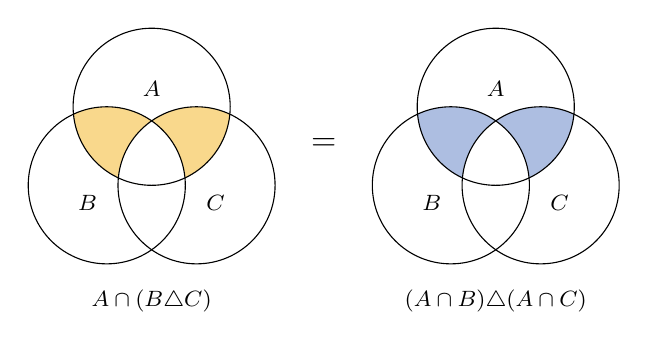
\begin{tikzpicture}[font=\footnotesize, scale=0.95]
\def\r{1.05}
\begin{scope}[shift={(0,0)}]
  \begin{scope}
    \clip (0,0.55) circle (\r);
    \begin{scope}
      \clip (-0.6,-0.5) circle (\r) (0.6,-0.5) circle (\r);
      \fill[armOrange!45] (-2,-2.2) rectangle (2,1.9);
    \end{scope}
    \begin{scope}
      \clip (-0.6,-0.5) circle (\r);
      \fill[white] (0.6,-0.5) circle (\r);
    \end{scope}
  \end{scope}
  \draw (0,0.55) circle (\r) node[above] {$A$};
  \draw (-0.6,-0.5) circle (\r) node[below left] {$B$};
  \draw (0.6,-0.5) circle (\r) node[below right] {$C$};
  \node at (0,-2.05) {$A\cap(B\symd C)$};
\end{scope}
\begin{scope}[shift={(4.6,0)}]
  \begin{scope}
    \clip (0,0.55) circle (\r);
    \begin{scope}
      \clip (-0.6,-0.5) circle (\r) (0.6,-0.5) circle (\r);
      \fill[armBlue!32] (-2,-2.2) rectangle (2,1.9);
    \end{scope}
    \begin{scope}
      \clip (-0.6,-0.5) circle (\r);
      \fill[white] (0.6,-0.5) circle (\r);
    \end{scope}
  \end{scope}
  \draw (0,0.55) circle (\r) node[above] {$A$};
  \draw (-0.6,-0.5) circle (\r) node[below left] {$B$};
  \draw (0.6,-0.5) circle (\r) node[below right] {$C$};
  \node at (0,-2.05) {$(A\cap B)\symd(A\cap C)$};
\end{scope}
\node at (2.3,0.05) {\large $=$};
\end{tikzpicture}
\end{center}

\answer{Երկու նույնություններն էլ ճիշտ են։ \ (3)՝ «$A$-ում կամ $B$-ում, $C$-ում ոչ» $=$ «$A$-ում, $C$-ում
ոչ» կամ «$B$-ում, $C$-ում ոչ»։ \ (11)՝ $x\in A$ լինել-չլինելը ֆիքսելուց հետո «$B,C$-ից ճիշտ մեկը»
համընկնում է «$A\cap B,A\cap C$-ից ճիշտ մեկին»։}

\begin{methodbox}
\textbf{Փոխանցելի տեխնիկա՝} ապացուցիր $X=Y$ տարրային հետապնդումով՝ բացիր $\cup,\cap,\setminus$-ը
«կամ / և / և ոչ»-ի և պարզեցրու տրամաբանությունը։ $\symd$-ով ամեն ինչի համար փոխարինիր այն «երկուսից
ճիշտ մեկում»-ով (զույգության պնդում), և եթե $A$-ի նման փոփոխականը հանդես է գալիս երկու կողմից, բաժանիր
$x\in A$ և $x\notin A$ դեպքերի։
\end{methodbox}

% ============================================================================
\section*{Խնդիր 58 - $A\times B=B\times A$-ն հարկադրում է $A=B$}

\begin{problembox}[58]
Ապացուցիր, որ $A\times B=B\times A$-ն հետևեցնում է $A=B$։
\end{problembox}

\begin{ideabox}
Արտադրյալի տարրը \emph{կարգավորված} զույգ է, և կարգն է, որ կրում է տեղեկությունը։ Եթե
$A\times B=B\times A$, ապա ցանկացած զույգ, որ կարող ես կազմել մի ձևով, պետք է արդեն հասանելի լինի մյուս
ձևով, և $(a,b)\in A\times B$-ի առաջին կոորդինատը $B\times A$-ի զույգերի առաջին կոորդինատի դեմ
համեմատելը հարկադրում է $a\in B$։ $A=B$ բազմությունների հավասարությունն ապացուցելու համար ցույց ենք
տալիս երկու պարունակում՝ $A\subseteq B$ և $B\subseteq A$։

Մեկ ազնիվ վերապահում, որ պնդումը թաքցնում է՝ պետք են $A$ և $B$ \emph{ոչ դատարկ}։ Եթե որևէ մեկը դատարկ է,
երկու արտադրյալներն էլ դատարկ են, և ենթադրությունը ճիշտ է ձրի՝ ոչինչ չասելով, ուստի եզրակացությունը
կարող է ձախողվել։ Նշում ենք հակաօրինակը, ապա ապացուցում պնդումը (նախատեսված) ոչ դատարկ ենթադրությամբ։
\end{ideabox}

\textbf{Քայլ 0 - Դատարկ բազմության եզրային դեպքը։}
Վերցրու $A=\varnothing$ և $B=\{1\}$։ Այդ դեպքում $A\times B=\varnothing$ և $B\times A=\varnothing$, ուստի
$A\times B=B\times A$-ն ճիշտ է, սակայն $A\neq B$։ Ուստի հետևությունը կարող է ձախողվել միայն երբ $A,B$-ից
\emph{ճիշտ մեկն} է դատարկ (եթե երկուսն էլ դատարկ են, այն ճիշտ է տրիվիալ կերպով, քանի որ այդ դեպքում
$A=B=\varnothing$)՝ այսուհետ ենթադրում ենք $A\neq\varnothing$ և $B\neq\varnothing$՝ միակ դեպքը, որ մնում
է փաստարկել։

\textbf{Քայլ 1 - Ցույց տուր $A\subseteq B$։}
Դիցուք $a\in A$ կամայական է։ Քանի որ $B\neq\varnothing$, ընտրիր ինչ-որ $b\in B$։ Այդ դեպքում
$(a,b)\in A\times B$։ Ենթադրությամբ $A\times B=B\times A$, ուստի $(a,b)\in B\times A$։ $B\times A$-ի
տարրն իր \emph{առաջին} կոորդինատն ունի $B$-ում; այդ առաջին կոորդինատը $a$ է, ուստի $a\in B$։ Քանի որ
$a\in A$-ն կամայական էր, $A\subseteq B$։

\textbf{Քայլ 2 - Ցույց տուր $B\subseteq A$։}
Սիմետրիկ կերպով, դիցուք $b\in B$ կամայական է։ Քանի որ $A\neq\varnothing$, ընտրիր ինչ-որ $a\in A$։ Այդ
դեպքում $(a,b)\in A\times B=B\times A$, և $B\times A$-ի տարրն իր \emph{երկրորդ} կոորդինատն ունի $A$-ում;
այդ երկրորդ կոորդինատը $b$ է, ուստի $b\in A$։ Հետևաբար $B\subseteq A$։

\textbf{Քայլ 3 - Եզրակացրու։}
$A\subseteq B$ և $B\subseteq A$ տալիս են $A=B$։ $\blacksquare$

\textbf{Ստուգում։} $\{0,1,2\}$-ի բոլոր ոչ դատարկ $A,B$ ենթաբազմությունների վրա ուղիղ որոնումը չի գտնում
ոչ մի զույգ՝ $A\times B=B\times A$ բայց $A\neq B$ պայմանով; իսկ դատարկ դեպքը $A=\varnothing$, $B=\{1\}$
իսկապես բավարարում է ենթադրությանը $A\neq B$-ով՝ ճիշտ ինչպես նշվեց։ \checkmark

\textbf{Ինչու՞ է փոխատեղումը հարկադրում $A=B$։} Գծիր յուրաքանչյուր զույգ որպես կետ։ $A=\{1,2\}$,
$B=\{3,4,5\}$-ով երկու արտադրյալները՝ $A\times B$-ն (կետեր $(a,b)$-ում) և $B\times A$-ն (կետեր
$(b,a)$-ում)՝ ընկնում են \emph{տարբեր} կետերի՝ դրանք նստած են հարթության տարբեր մասերում և չեն կարող
համընկնել, քանի դեռ $A$-ն և $B$-ն նույն թվերի բազմությունը չեն՝

\begin{center}
\begin{tikzpicture}[font=\footnotesize, scale=0.62, >=Stealth]
\begin{scope}
  \draw[->] (0,0) -- (6.3,0) node[right] {1-ին կոորդ.};
  \draw[->] (0,0) -- (0,6.3) node[above] {2-րդ կոորդ.};
  \foreach \x in {1,2,3,4,5}{\draw (\x,0.08)--(\x,-0.08) node[below]{$\x$};}
  \foreach \y in {1,2,3,4,5}{\draw (0.08,\y)--(-0.08,\y) node[left]{$\y$};}
  \foreach \a in {1,2}\foreach \b in {3,4,5}{\fill[armRed] (\a,\b) circle (3.2pt);}
  \node[armRed] at (3.1,5.7) {$A\times B$};
  \node at (3.0,-1.3) {կետեր $(a,b)$-ում, $a\in A,\ b\in B$};
\end{scope}
\begin{scope}[shift={(8.3,0)}]
  \draw[->] (0,0) -- (6.3,0) node[right] {1-ին կոորդ.};
  \draw[->] (0,0) -- (0,6.3) node[above] {2-րդ կոորդ.};
  \foreach \x in {1,2,3,4,5}{\draw (\x,0.08)--(\x,-0.08) node[below]{$\x$};}
  \foreach \y in {1,2,3,4,5}{\draw (0.08,\y)--(-0.08,\y) node[left]{$\y$};}
  \foreach \b in {3,4,5}\foreach \a in {1,2}{\draw[armBlue, thick, fill=white] (\b,\a) circle (3.2pt);}
  \node[armBlue] at (4.3,5.7) {$B\times A$};
  \node at (3.0,-1.3) {կետեր $(b,a)$-ում, $b\in B,\ a\in A$};
\end{scope}
\end{tikzpicture}
\end{center}
Կարմիր և կապույտ կետերի բազմությունները անկյունագծի նկատմամբ արտապատկերումներ են; դրանք համընկնում են
միայն անկյունագծի վրա, ուստի $A\times B=B\times A$-ն կարող է տեղի ունենալ միայն երբ $A=B$։

\answer{Ոչ դատարկ $A,B$-ի համար՝ $A\times B=B\times A\Rightarrow A=B$, ապացուցված երկու պարունակումներով։
Ոչ դատարկությունը անհրաժեշտ է՝ $A=\varnothing$, $B=\{1\}$ հակաօրինակ է առանց դրա։}

\begin{methodbox}
\textbf{Փոխանցելի տեխնիկա՝} $A=B$ բազմությունների հավասարությունն ապացուցելու համար ապացուցիր
$A\subseteq B$ և $B\subseteq A$ առանձին («վերցրու կամայական տարր, ցույց տուր, որ այն մյուսում է»)։ Երբ
արտադրյալներ են հանդես գալիս, կարդա այն կոորդինատը, որ կրում է տեղեկությունը՝ $X\times Y$-ի զույգի առաջին
կոորդինատը $X$-ում է, երկրորդը՝ $Y$-ում։ Եվ միշտ ստուգիր «ակնհայտ» հետևությունը դատարկ բազմության վրա՝
նախքան դրան վստահելը։
\end{methodbox}

% ============================================================================
\section*{Խնդիր 60 - Դեկարտյան արտադրյալի բաշխական օրենքները}

\begin{problembox}[60]
Ապացուցիր (1)-(6) նույնությունները՝
\begin{enumerate}[label=\textbf{(\arabic*)},leftmargin=1.4cm,itemsep=1pt]
\item $A\times(B\cup C)=(A\times B)\cup(A\times C)$;
\item $(B\cup C)\times A=(B\times A)\cup(C\times A)$;
\item $A\times(B\cap C)=(A\times B)\cap(A\times C)$;
\item $(B\cap C)\times A=(B\times A)\cap(C\times A)$;
\item $A\times(B\setminus C)=(A\times B)\setminus(A\times C)$;
\item $(B\setminus C)\times A=(B\times A)\setminus(C\times A)$.
\end{enumerate}
\end{problembox}

\begin{ideabox}
Արտադրյալի յուրաքանչյուր տարր կարգավորված զույգ է $(x,y)$, և «$(x,y)\in X\times Y$»-ն պարզապես
«$x\in X$ \emph{և} $y\in Y$» կոնյունկցիան է։ Ուստի հենց որ գրում ես $(x,y)$ և բացում ես երկու կողմերը
առանձին $x$-ի և $y$-ի մասին պնդումների, յուրաքանչյուր նույնություն դառնում է ասույթային տրամաբանության
փոքրիկ կտոր՝ $\cup$-ն «կամ» է $y$-մասի վրա, $\cap$-ն «և», $\setminus$-ը «և ոչ», իսկ ֆիքսված $x\in A$
արտադրիչը պարզապես անփոփոխ ուղեկցում է։ Ապացուցիր (1), (3), (5)-ը այս կարգավորված-զույգ ${\iff}$ մեթոդով;
(2), (4), (6)-ը \emph{նույն} ապացույցներն են արտադրյալը մյուս կողմում՝ փոխիր կոորդինատների դերերը։
\end{ideabox}

\textbf{(1) Միավորում աջ արտադրիչի վրա։}
\begin{align*}
(x,y)\in A\times(B\cup C)
&\iff x\in A\ \text{և}\ (y\in B\ \text{կամ}\ y\in C)\\
&\iff (x\in A\ \text{և}\ y\in B)\ \text{կամ}\ (x\in A\ \text{և}\ y\in C)
   &&\text{[բաշխիր «և»-ը «կամ»-ի վրա]}\\
&\iff (x,y)\in A\times B\ \text{կամ}\ (x,y)\in A\times C\\
&\iff (x,y)\in(A\times B)\cup(A\times C). \qquad\blacksquare
\end{align*}

\textbf{(3) Հատում աջ արտադրիչի վրա։} Նույն հետապնդումը «և»-ով՝
\begin{align*}
(x,y)\in A\times(B\cap C)
&\iff x\in A\ \text{և}\ y\in B\ \text{և}\ y\in C\\
&\iff (x\in A\ \text{և}\ y\in B)\ \text{և}\ (x\in A\ \text{և}\ y\in C)
   &&\text{[$x\in A$-ն ազատ կրկնվում է]}\\
&\iff (x,y)\in(A\times B)\cap(A\times C). \qquad\blacksquare
\end{align*}

\textbf{(5) Տարբերություն աջ արտադրիչի վրա։}
\begin{align*}
(x,y)\in A\times(B\setminus C)
&\iff x\in A\ \text{և}\ y\in B\ \text{և}\ y\notin C.
\end{align*}
Մյուս կողմում,
$$(x,y)\in(A\times B)\setminus(A\times C)\iff (x\in A\ \text{և}\ y\in B)\ \text{և}\ \neg(x\in A\ \text{և}\ y\in C).$$
Բայց առաջին հատվածն արդեն տալիս է $x\in A$, ուստի $\neg(x\in A\ \text{և}\ y\in C)$-ն փլուզվում է
$y\notin C$-ի։ Հետևաբար սա $x\in A$ և $y\in B$ և $y\notin C$ է՝ նույնական վերևի տողին։ Ուստի երկու
բազմությունները հավասար են։ $\blacksquare$

\textbf{(2), (4), (6) - հայելային պատկերները։}
Սրանք (1), (3), (5)-ն են $A$ փոփոխական արտադրիչը \emph{առաջին} կոորդինատ տեղափոխած։ Կիրառիր նույն
փաստարկը $(y,x)$ զույգի վրա $(y,x)\in X\times A\iff y\in X$ և $x\in A$-ով; ֆիքսված մասն այժմ $x\in A$ է
երկրորդ դիրքում, և $\cup,\cap,\setminus$-ը բաշխվում են $y$-մասի վրա ճիշտ ինչպես առաջ։ Կոնկրետ՝
\begin{align*}
(y,x)\in(B\cup C)\times A &\iff (y\in B\ \text{կամ}\ y\in C)\ \text{և}\ x\in A
  \iff (y,x)\in(B\times A)\cup(C\times A),\\
(y,x)\in(B\cap C)\times A &\iff y\in B\ \text{և}\ y\in C\ \text{և}\ x\in A
  \iff (y,x)\in(B\times A)\cap(C\times A),\\
(y,x)\in(B\setminus C)\times A &\iff y\in B\ \text{և}\ y\notin C\ \text{և}\ x\in A
  \iff (y,x)\in(B\times A)\setminus(C\times A).\qquad\blacksquare
\end{align*}

\textbf{Ստուգում։} Բոլոր վեց նույնությունները ստուգվեցին $\{0,1,2\}$-ի $A,B,C$ ենթաբազմությունների
յուրաքանչյուր եռյակի վրա ուղիղ թվարկումով (ուստի յուրաքանչյուր հնարավոր արտադրյալ համեմատվեց վանդակ առ
վանդակ)՝ \emph{զրո} անհամապատասխանություն։ \checkmark

\textbf{Բաշխական օրենք (1)-ը որպես մակերեսի պատկեր։} Գծիր $A$-ն որպես միջակայք $x$-առանցքի վրա, իսկ $B$,
$C$-ն որպես երկու դարսված շերտ $y$-առանցքի վրա։ $X\times Y$ արտադրյալը «$X$-ի վրա, $Y$-ի կողքին»
ուղղանկյունն է։ Այդ դեպքում $A\times(B\cup C)$-ն $A$-ի վրա ամբողջ բլոկն է՝ ընդգրկելով $B$-ն և $C$-ն,
ինչը հենց $A\times B$ ուղղանկյունն է՝ $A\times C$ ուղղանկյան վրա դարսված՝

\begin{center}
\begin{tikzpicture}[font=\footnotesize, scale=0.9, >=Stealth]
\draw[->] (0,0) -- (6.4,0) node[right] {առաջին կոորդինատ};
\draw[->] (0,0) -- (0,4.3) node[above] {երկրորդ կոորդինատ};
\draw[armOrange!85!black, line width=2.4pt] (1,0) -- (3.2,0);
\node[armOrange!75!black, anchor=north] at (2.1,-0.12) {$A$};
\draw[armRed!85!black, line width=2.4pt] (0,0.6) -- (0,1.9);
\node[armRed!75!black, anchor=east] at (-0.08,1.25) {$B$};
\draw[armBlue!85!black, line width=2.4pt] (0,2.2) -- (0,3.6);
\node[armBlue!75!black, anchor=east] at (-0.08,2.9) {$C$};
\fill[armRed!22] (1,0.6) rectangle (3.2,1.9);
\draw[armRed!75!black] (1,0.6) rectangle (3.2,1.9);
\node[armRed!75!black] at (2.1,1.25) {$A\times B$};
\fill[armBlue!20] (1,2.2) rectangle (3.2,3.6);
\draw[armBlue!75!black] (1,2.2) rectangle (3.2,3.6);
\node[armBlue!75!black] at (2.1,2.9) {$A\times C$};
\draw[decorate, decoration={brace, amplitude=5pt}, gray!55!black] (3.55,3.6) -- (3.55,0.6);
\node[gray!55!black, anchor=west, align=left] at (3.75,2.1)
  {$A\times(B\cup C)$\\[1pt]$=(A\times B)\cup(A\times C)$};
\end{tikzpicture}
\end{center}

\answer{Բոլոր վեցն էլ ճիշտ են։ Աջ-արտադրիչ օրենքները (1),(3),(5) հետևում են
$(x,y)\in X\times Y\iff x\in X\wedge y\in Y$-ից՝ բաշխելով բազմության գործողությունը $y$-կոորդինատի վրա,
մինչդեռ $x\in A$-ն ուղեկցում է; ձախ-արտադրիչ օրենքները (2),(4),(6) նույնն են կոորդինատները փոխած։}

\begin{methodbox}
\textbf{Փոխանցելի տեխնիկա՝} դեկարտյան արտադրյալը բազմությունների հանրահաշիվը վերածում է կոորդինատների
տրամաբանության՝ $(x,y)\in X\times Y\iff (x\in X)\wedge(y\in Y)$։ Արտադրյալի նույնություն ապացուցելու
համար գրիր ընդհանուր $(x,y)$ զույգ, բացիր երկու կողմերը երկու կոորդինատների մասին «և/կամ/ոչ» պնդումների, և
օգտագործիր սովորական տրամաբանական բաշխում։ Հաստատուն արտադրիչը (այստեղ $A$) պարզապես հանդես է գալիս՝
անփոփոխ, նույն կոորդինատում երկու կողմից։
\end{methodbox}

\end{document}
